% $Id: INF_Poster_example.tex 7714 2011-08-31 17:34:46Z tkren $
%
% TU Wien - Faculty of Informatics
% poster template
%
% This template is using the beamer document class and beamerposter package, see
% <http://www.ctan.org/tex-archive/macros/latex/contrib/beamer/>
% <http://www.ctan.org/tex-archive/macros/latex/contrib/beamerposter/>
% <http://www-i6.informatik.rwth-aachen.de/~dreuw/latexbeamerposter.php>
%
% For questions and comments send an email to
% Thomas Krennwallner <tkren@kr.tuwien.ac.at>
%

\documentclass[final,hyperref={pdfpagelabels=true}]{beamer}

\usepackage{minted}
%\usepackage{ucs}
\usepackage{TUINFPST}
\usepackage{listings}
\usepackage{wrapfig}
\usepackage{comment}

\usepackage[scaled]{beramono}
\fvset{fontsize=\normalsize}

\usemintedstyle{perldoc}

%\usepackage{ucs}

%\title[Computational Intelligence]{Interactive Computer Generated Architecture}
% if you have a long title looking squeezed on the poster, just force
% some distance:
\title[Software Engineering \& Internet Computing]{%
  A Weather Ontology for \\[0.2\baselineskip]%
  Predictive Control in Smart Homes %\\[0.2\baselineskip]%
}
\author[paulchen@rueckgr.at]{Paul Staroch}
\institute[]{%
  Technische Universit{\"a}t Wien\\[0.25\baselineskip]
  Institut für Rechnergestützte Automation\\[0.25\baselineskip]
  Arbeitsbereich: Automatisierungssysteme\\[0.25\baselineskip]
  Betreuer: Ao.Univ.-Prof. Dipl.-Ing. Dr.techn. Wolfgang Kastner\\[0.25\baselineskip]
  Assistent: Dipl.-Ing. Mario Kofler
}
\titlegraphic{\includegraphics[height=52mm]{figures/183-1.pdf}}
\date[\today]{\today}
\subject{epilog}
\keywords{my kwd1, my kwd2} % TODO

%%%%%%%%%%%%%%%%%%%%%%%%%%%%%%%%%%%%%%%%%%%%%%%%%%%%%%%%%%%%%%%%%%%%%%%%%%%%%%%%%%%%%%

% Display a grid to help align images 
%\beamertemplategridbackground[12.7mm] % TODO remove

% play around with the background colors
%\setbeamercolor{background canvas}{bg=yellow}

% use a background picture
\usebackgroundtemplate{%
  \includegraphics[width=\paperwidth]{figures/ap51514966743ad_full.jpg}
}

% play around with block colors
\setbeamercolor{block body}{fg=black,bg=white}
\setbeamercolor{block title}{fg=TuWienBlue,bg=white}

\definecolor{TuWienBlueLight}{cmyk}{.1,.1,.1,.3}
\definecolor{listingBottom}{cmyk}{.1,.1,.1,.1}

\setbeamertemplate{block begin}{
  \pgfsetfillopacity{0.7}
  \begin{beamercolorbox}{block title}%
    \begin{tikzpicture}%
      \node[draw,rectangle,line width=3pt,rounded corners=0pt,inner sep=0pt,shade,top color=white,bottom color=TuWienBlueLight]{%
        \begin{minipage}[c][2cm]{\linewidth}
          \centering\textbf{\insertblocktitle}
        \end{minipage}
      };
    \end{tikzpicture}%
  \end{beamercolorbox}
  \begin{beamercolorbox}[colsep=1.5pt,sep=1cm]{block body}%
%  \vspace*{.5cm}
}

\setbeamertemplate{block end}{
  \end{beamercolorbox}
  \vspace{1cm}
}

% setup postit
\setbeamercolor{postit}{fg=black,bg=yellow} 
\newenvironment{postit}
{\begin{beamercolorbox}[sep=1em,wd=7cm]{postit}}
{\end{beamercolorbox}}


% for crop marks, uncomment the following line
\usepackage[cross,width=88truecm,height=123truecm,center]{crop} % TODO

%%%%%%%%%%%%%%%%%%%%%%%%%%%%%%%%%%%%%%%%%%%%%%%%%%%%%%%%%%%%%%%%%%%%%%%%%%%%%%%%%%%%%%

%\lstset{frame=trbl,basicstyle=\scriptsize,moredelim=**[is][{\btHL[fill=green!20]}]{@@}{@@},}
%\lstset{frame=trBL,basicstyle=\normalsize}

% \setlength{\parskip}{15em}

% \addtobeamertemplate{block begin}{\pgfsetfillopacity{0.5}}{\pgfsetfillopacity{1}}

\begin{document}

% We have a single poster frame.
\begin{frame}[fragile]
  \begin{columns}[t]
    % ---------------------------------------------------------%
    % Set up a column
    \begin{column}{.45\textwidth}
      \begin{block}{Smart homes and ontologies}
        \begin{wrapfigure}{r}{.45\textwidth}
	  \centering
	  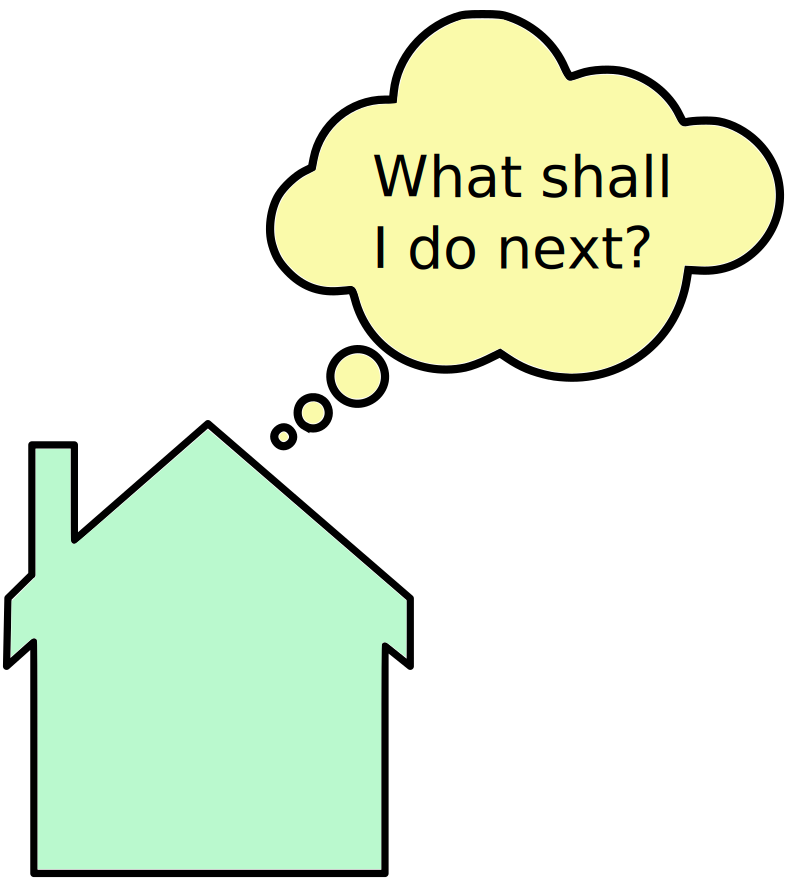
\includegraphics[width=.35\textwidth]{figures/inkscape/smart_home}
	  \vspace{4cm}
	\end{wrapfigure}

	\vspace{-1.5em}
	
	\emph{Smart homes} are dwellings that
	
	\begin{itemize}
	  \item \mbox{are equipped with some kind} of intelligence.
	  \item perform tasks on their own.
	\end{itemize}

	\vspace{.5em}
	Some of their goals are:

	\begin{itemize}
	  \item \mbox{Support the inhabitants in their} routine tasks.
	  \item Maintain or increase comfort.
          \item Reduce the energy consumption.
        \end{itemize}

	\vspace{.5em}
        Problems of many smart home systems:

        \begin{itemize}
	  \item High complexity.
	  \item Optimising and customising are difficult.
	  \item Missing powerfulness and flexibility.
	\end{itemize}

	\vspace{.5em}
	To overcome these problems, a knowledge
	base built using \emph{OWL} can be introduced.
      \end{block}

      \begin{block}{Why introduce a weather data model?}
        \begin{wrapfigure}{r}{.55\textwidth}
	  \centering
	  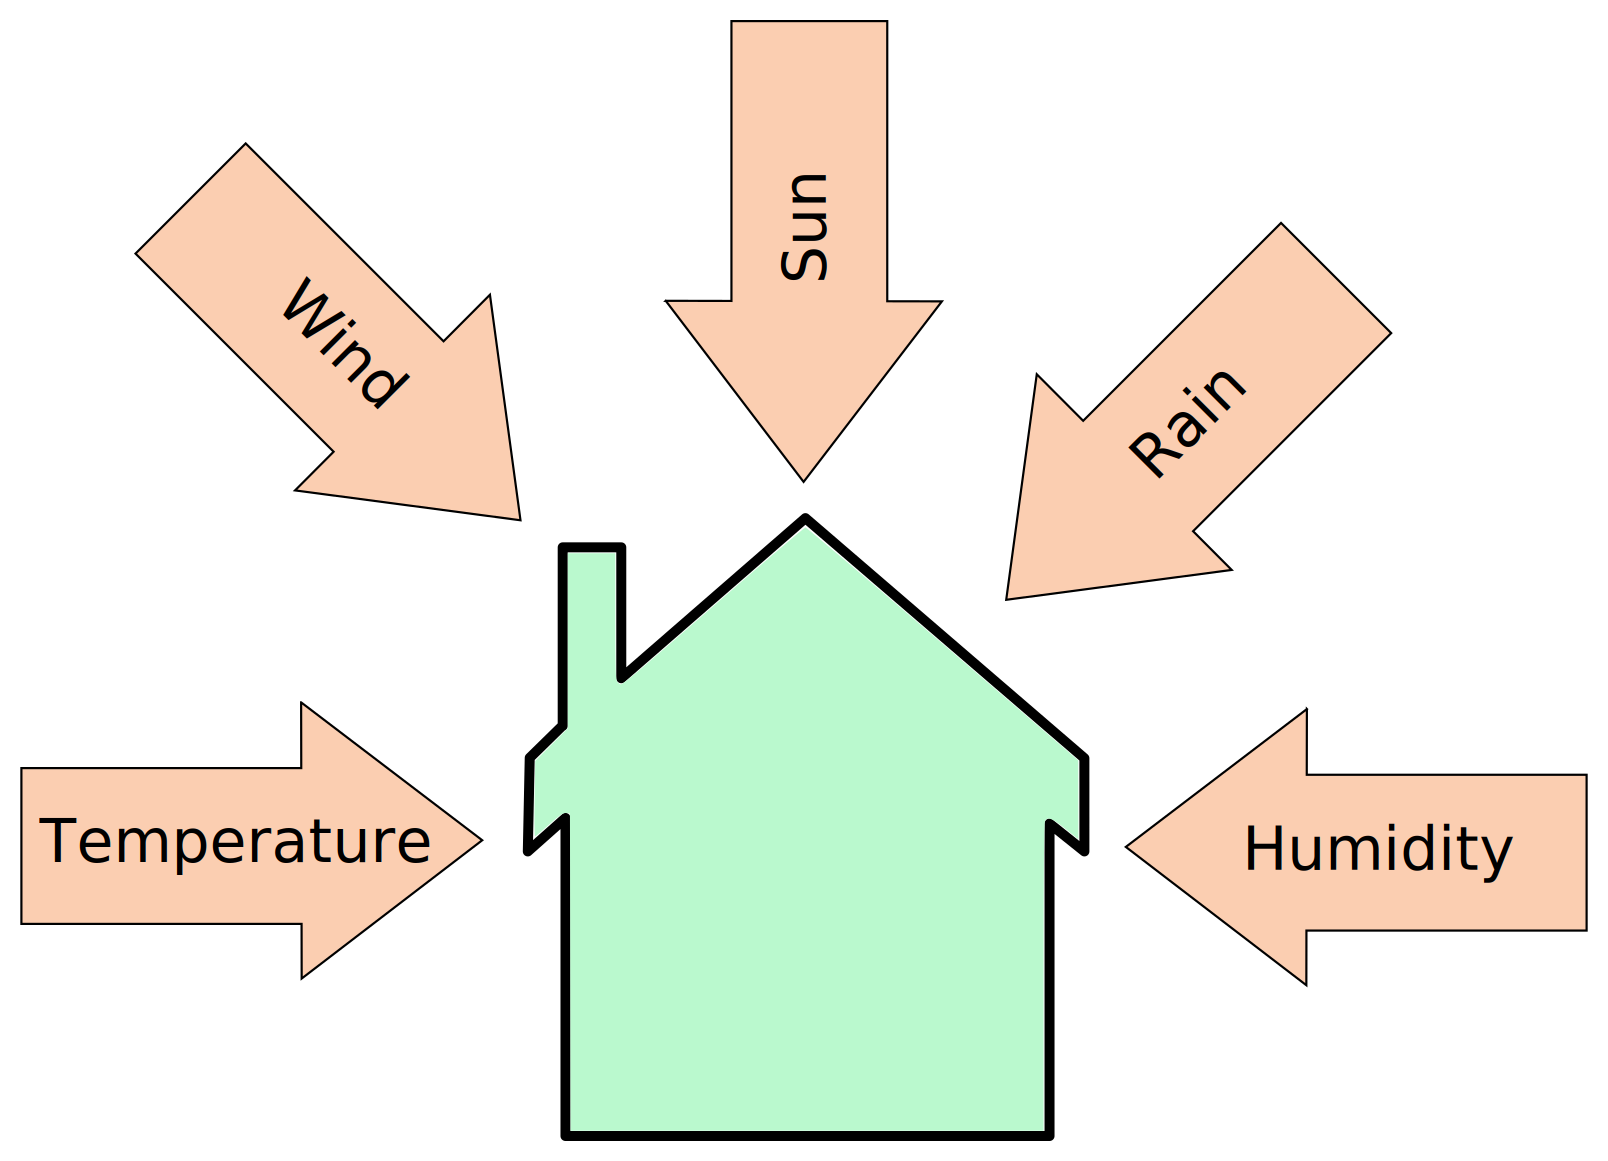
\includegraphics[width=.46\textwidth]{figures/inkscape/house}
	  \vspace{4cm}
	\end{wrapfigure}

	\vspace{-1.5em}
	
	\mbox{Weather has a wide influence on}
	\mbox{a dwelling. \emph{SmartHomeWeather}}
	
	\begin{itemize}
	  \item is an ontological data model.
	  \item supports current and future weather data.
	  \item enables a smart home to make weather-based control decisions.
	\end{itemize}

	\vspace{.5em}
	Examples for such control decisions:
	
	\begin{itemize}
  	  \item Heating, ventilation, and air conditioning (\emph{HVAC}),
	  \item Utilisation of solar and wind power.
	  \item Irrigation.
	  \item Preparing for severe weather (e.g. close windows, retract awnings).
	\end{itemize}

	\vspace{.5em}
	Data about weather states are obtained from local sensors and Internet weather services.
      \end{block}

      \begin{block}{Methodological approach}
	The preliminary work included:
	\begin{itemize}
	  \item Evaluation of existing weather ontologies.
	  \item Identification of uses cases for weather data in smart homes.
	  \item Analysis of methodologies for ontology design.
	  \item Examination of sources for weather data (sensors and Internet services).
	\end{itemize}
	
	\vspace{.5em}
	Based on this knowledge, the following steps were performed:
	
	\begin{itemize}
	  \item Design of \emph{SmartHomeWeather} using \emph{METHONTOLOGY}. % ~\cite{Methontology}.
	  \item Development of \emph{Weather Importer}.
	\end{itemize}
      \end{block}

      \begin{block}{The \emph{SmartHomeWeather} ontology}
	\begin{itemize}
	  \item The \emph{SmartHomeWeather} ontology is built around five top-level concepts.
	  \item Each top-level concept is root of a concept hierarchy.
	  \item \emph{OWL} reasoning is heavily used.
	\end{itemize}
      \end{block}
    \end{column}
    % ---------------------------------------------------------%
    % end the column

    % ---------------------------------------------------------%
    % Set up a column 
    \begin{column}{.45\textwidth}
      \begin{block}{The \emph{SmartHomeWeather} ontology (cont.)}
	\includegraphics[width=\textwidth-2cm]{figures/dia/binary-relations}
	\begin{itemize}
	  \item \emph{Weather phenomenon}: A certain weather
		  element: temperature, humidity, …
	  \item \emph{Weather condition}: A one-word description of the
		  weather situation: ``Sun'', ``Fog'', …
	  \item \emph{Weather state}: The weather situation as a
		  set of \emph{Weather phenomena}.
          \item \emph{Weather report}: The weather for one
		  point of time.
	  \item \emph{Weather report source}: A source of weather data
		  (sensor or Internet service)
	\end{itemize}

	\vspace{.5em}
	
	This is a part of the concept hierarchy of \emph{Weather phenomenon}:
	
	\vspace{1em}
	\includegraphics[width=\textwidth-2cm]{figures/dia/hierarchy}

	\vspace{.5em}
	Querying the data model is done using \emph{SPARQL} queries:

	\vspace{10mm}
	\begin{tikzpicture}%
          \node[draw,rectangle,line width=3pt,rounded corners=0pt,inner sep=0pt,shade,top color=white,bottom color=listingBottom]{%
	    \begin{minipage}{\dimexpr\textwidth-2cm}
	      \hspace{5mm}
              \begin{minipage}{\dimexpr\textwidth-2cm}
              \vspace{10mm}
    	      \begin{minted}{sparql}
SELECT ?r
WHERE {
    ?r weather:hasWeatherState ?s.
    ?s weather:hasWeatherPhenomenon ?t.
    ?t a weather:RoomTemperature.
}
    	      \end{minted}
    	      \vspace{5mm}
	      \end{minipage}
            \end{minipage}
	  };
	\end{tikzpicture}
	\vspace{-12mm}
	
	The Java application \emph{Weather Importer} retrieves weather data from sensors and services into \emph{SmartHomeWeather}.
      \end{block}
      
      \begin{block}{Future work}
	\begin{itemize}
	  \item Identification of further use cases of \emph{SmartHomeWeather}.
	  \item Interoperation with other data sources, e.g.:
	    \begin{itemize}
	      \item Minimising costs for electrical power based on weather data and varying costs for electrical power over time.
	      \item Improving decision making based on both weather data and the buildings' inhabitants' actions.
	      \item Learning from weather situations and their influence on the dwelling.
	    \end{itemize}
	\end{itemize}
      \end{block}

%      \begin{block}{References}
%        \footnotesize
%	\bibliographystyle{thesis}
%	\bibliography{references}
%      \end{block}
    \end{column}
    % ---------------------------------------------------------%
    % end the column
  \end{columns}

%  \begin{tikzpicture}[remember picture,overlay]
%    \node[inner sep=0pt,xshift=-30cm,yshift=23cm] at (current page.east) {%
%      \begin{postit}%
%        Post-It time!%
%      \end{postit}%
%    }; 
%  \end{tikzpicture}
  
\end{frame}

\end{document}


%%% Local Variables:
%%% TeX-PDF-mode: t
%%% TeX-debug-bad-boxes: t
%%% TeX-master: t
%%% TeX-parse-self: t
%%% TeX-auto-save: t
%%% reftex-plug-into-AUCTeX: t
%%% End:
